% !TeX root = 系统动力学建模与仿真笔记.tex
\section{多刚体系统的元件组成}

本章的目标是给出组装多刚体系统动力学方程所需的全部元件级要素：广义坐标、约束方程及其雅可比矩阵、广义质量矩阵、动能与势能对广义坐标的偏导数. 为此，首先需要建立多刚体系统的描述框架——将系统拆分为基本元件，再按拓扑关系组装.

多刚体系统传递矩阵法采用元件化思想进行描述：系统由大地元件、$n$ 个体元件以及 $m$ 个铰元件组成，各元件统一编号，各自携带描述自身属性的参数与广义坐标，系统的总体方程由各元件的贡献按拓扑连接关系组装得到. 其中，体元件对应"物质"，承载系统的惯性属性；铰元件对应"连接"，规定相邻体元件之间允许的相对运动.

体元件是刚体的理想化模型，承载系统的质量、质心位置与转动惯量等惯性属性，其位形由连体坐标系相对于全局惯性坐标系的广义坐标描述；大地元件可视为编号为 0 的特殊体元件，其连体坐标系即全局惯性坐标系（0 系）. 体元件与大地元件之间同样通过铰元件相连，如图~\ref{fig:与大地关联的体元件}~所示.

\begin{figure}[htbp]
    \centering
    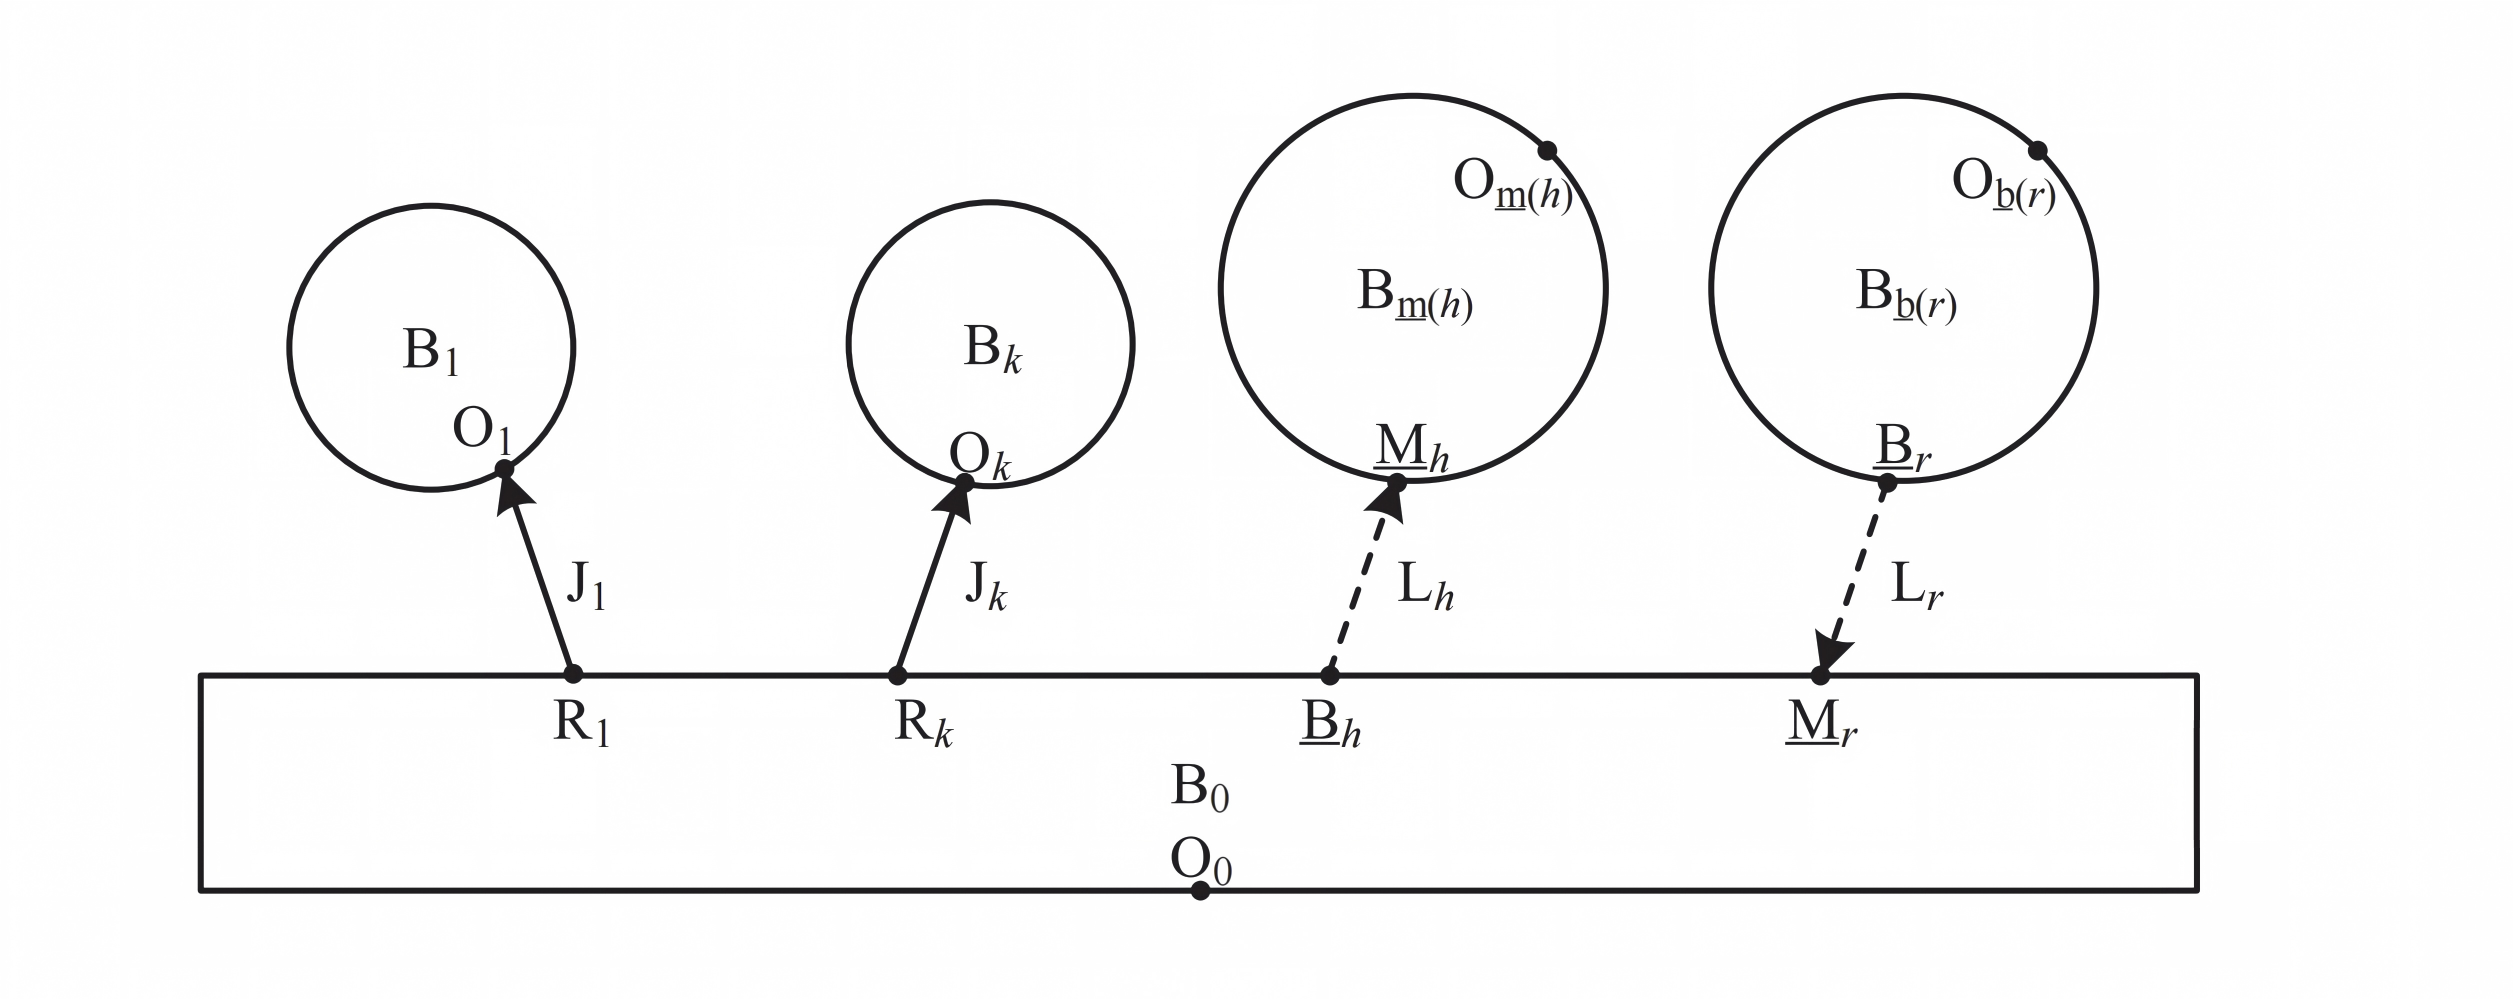
\includegraphics[width=0.8\textwidth]{Figure/与大地关联的体元件.png}
    \caption{与大地关联的体元件}
    \label{fig:与大地关联的体元件}
\end{figure}

铰元件是体元件之间运动副连接的理想化数学抽象：将轴承、销轴、导轨、万向节等物理连接零件忽略质量，并理想化为无间隙、无摩擦、无弹性，即得到相应的铰元件模型. 铰元件本身不计质量、不占几何体积，仅承担两项职责：限制被连两体元件之间的相对运动，以及作为相对运动的载体传递相邻体元件之间的运动学量. 一个铰元件 $\text{J}_j$ 由三方面要素完全确定：
\begin{enumerate}
    \item 关联的两个体元件，即 $\underline{\text{b}}(j)$ 体上的点 $\underline{\text{B}}_j$ 与 $\underline{\text{m}}(j)$ 体上的点 $\underline{\text{M}}_j$，该体对编号承载系统的拓扑连接信息；
    \item 几何锚点，即两个铰点在各连体坐标系中的定常位置矢量；
    \item 允许的相对运动形式，如转动铰元件的转轴方向单位矢量 $\bm{n}_{\text{J}_j}$.
\end{enumerate}
如图所示：

\begin{figure}[htbp]
    \centering
    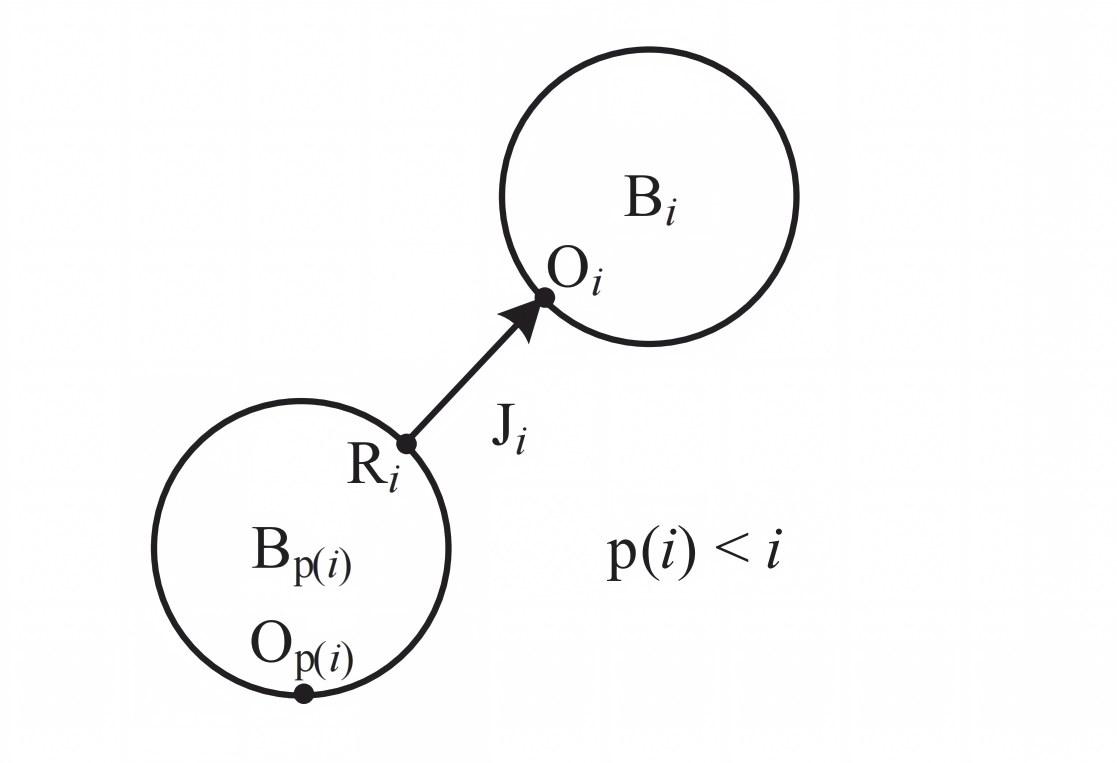
\includegraphics[width=0.5\textwidth]{Figure/非切断铰及其关联的体元件.png}
    \caption{示意图}
    \label{fig:非切断铰及其关联的体元件}
\end{figure}

图~\ref{fig:非切断铰及其关联的体元件}~为未切断铰元件时系统作为整体连接的情形；与之对照，将各铰元件切断，系统即分解为若干通过切口相互关联的体元件，如图~\ref{fig:切断铰及其关联的体元件}~所示. 这种“切断—组装”的处理是按元件列写方程、再按拓扑连接关系组装系统总体方程的基础.

\begin{figure}[htbp]
    \centering
    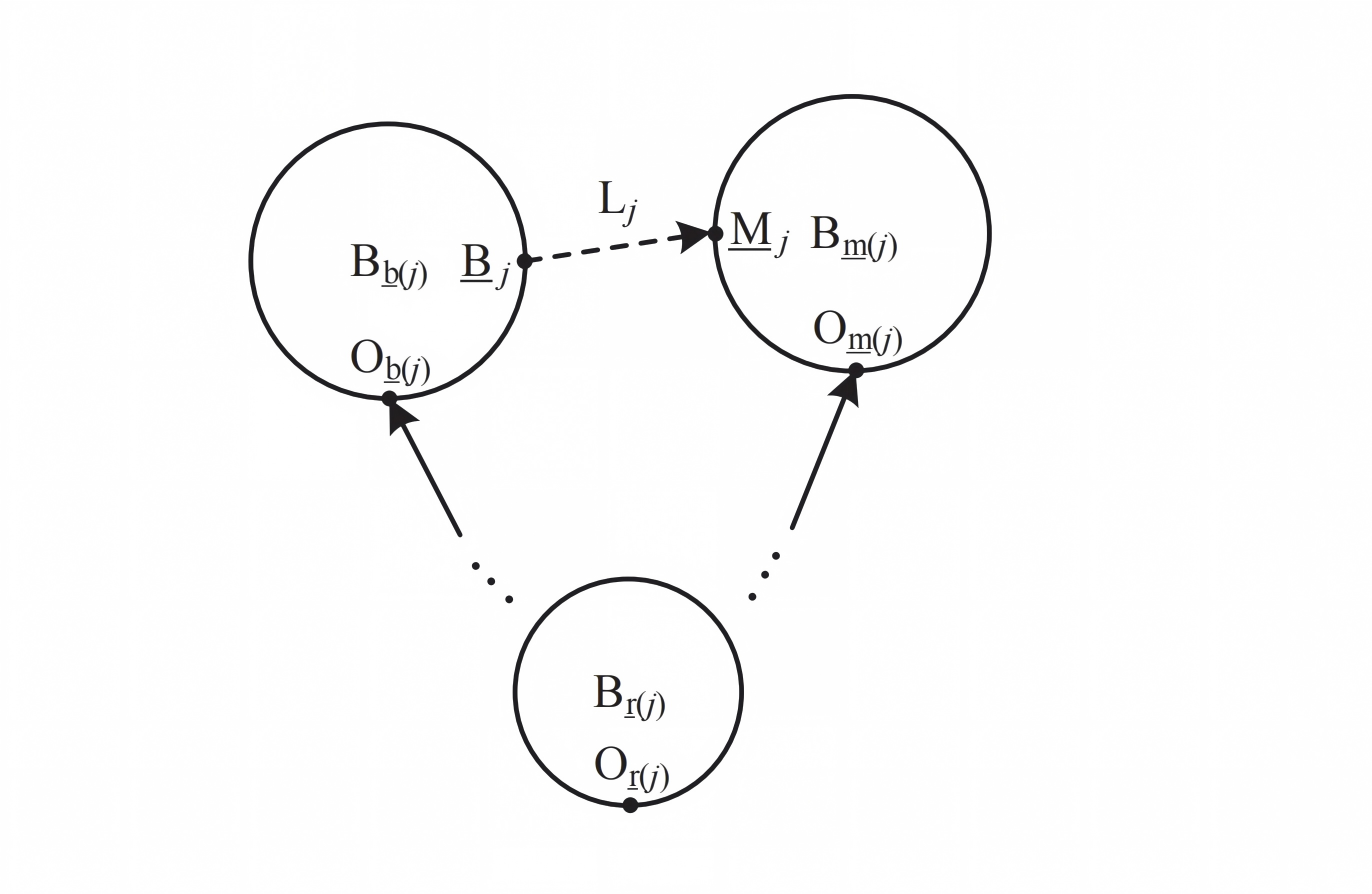
\includegraphics[width=0.5\textwidth]{Figure/切断铰及其关联的体元件.png}
    \caption{切断铰及其关联的体元件}
    \label{fig:切断铰及其关联的体元件}
\end{figure}

按允许的相对运动形式，常见铰元件及其位置级约束方程条数如下表所示：

\begin{center}
\begin{tabular}{ccc}
    \hline
    铰元件类型 & 允许的相对运动 & 位置级约束方程条数 \\
    \hline
    固接元件 & 无 & $6$ \\
    转动铰元件 & $1$ 个相对转动 & $5$ \\
    滑移铰元件 & $1$ 个相对平移 & $5$ \\
    万向节元件 & $2$ 个相对转动 & $4$ \\
    圆柱铰元件 & $1$ 个相对转动与 $1$ 个相对平移 & $4$ \\
    球铰元件 & $3$ 个相对转动 & $3$ \\
    \hline
\end{tabular}
\end{center}

表中约束方程条数等于 $6$ 减去允许的相对自由度个数，即每个铰元件削去相应个数的系统自由度. 铰元件在后续章节中承担三种角色：在本章系统约束方程中作为跨体耦合约束的来源，提供约束方程族 $\bm{c}_{\text{J}}$；在树形多刚体系统递推建模中，每个铰元件关联一组相对广义坐标 $\bm{q}_{\text{J}_i}$，使铰约束被坐标选取自动满足；在系统动力学方程中，铰元件约束反力以拉格朗日乘子的形式进入方程.

\section{多刚体系统体元件广义坐标}

有了元件化框架，接下来需要为每个体元件选取广义坐标. 描述一个刚体的空间位形需要 6 个独立量：3 个确定平动（原点位置），3 个确定转动（姿态角度）. 因此，每个体元件的广义坐标取为 6 维向量：前 3 个分量描述体坐标系原点在全局惯性系中的位置，后 3（或 4）个分量描述体坐标系相对全局惯性系的转动. 具体来说，多刚体系统体元件广义坐标 $\bm{q}$ 由系统中所有体元件连体坐标系相对于全局惯性坐标系的广义坐标构成，可记为
\begin{equation}
    \bm{q} = \begin{bmatrix} \bm{q}_{\text{B}_1}^\text{T} & \bm{q}_{\text{B}_2}^\text{T} & \cdots & \bm{q}_{\text{B}_n}^\text{T} \end{bmatrix}^\text{T},
\end{equation}
式中 $n$ 表示系统包含的体元件个数；$\bm{q}_{\text{B}_i}$ $(i = 1, 2, \cdots, n)$ 表示体元件 $i$ 连体坐标系相对于全局惯性坐标系的广义坐标，可表示为
\begin{equation}
    \bm{q}_{\text{B}_i} = \begin{bmatrix} \bm{r}_{\text{O}_0\text{O}_i|0}^\text{T} & \bm{\theta}_{0,i}^\text{T} \end{bmatrix}^\text{T},
\end{equation}
式中 $\bm{r}_{\text{O}_0\text{O}_i|0}$ 表示从全局惯性坐标系（0 系）原点 $\text{O}_0$ 到体元件 $i$ 连体坐标系（$i$ 系）原点 $\text{O}_i$ 的位置矢量在 0 系中的投影列阵；$\bm{\theta}_{0,i}$ 表示 $i$ 相对于 0 系的相对转动广义坐标，可取为欧拉四元数或三轴角形式。

\section{系统约束方程}

Recall from §1 that each body element $i$ is assigned a set of generalized coordinates $\bm{q}_{\text{B}_i} = [\bm{r}_{\text{O}_0\text{O}_i|0}^\text{T},\, \bm{\theta}_{0,i}^\text{T}]^\text{T}$ describing the position and orientation of its body-fixed frame relative to the global inertial frame. Physically, a free rigid body in three-dimensional space has exactly 6 independent degrees of freedom---3 for translation and 3 for rotation---and $\bm{q}_{\text{B}_i}$ captures precisely these 6 quantities (or 7, when Euler parameters are used to represent the 3 rotational degrees of freedom).

In a multi-body system, however, the body elements are not free: they are connected by hinge elements, as described in §1. Each hinge restricts certain relative motions between the two bodies it joins. The purpose of this section is to write these restrictions as algebraic equations---the constraint equations---and to compute their derivatives with respect to the generalized coordinates, which will later enter the Lagrange-multiplier formulation of the equations of motion.

\subsection{总体约束方程的结构}

The constraint equations of the system arise from two distinct sources, and it is important to keep them separate.

The first source is the hinge elements themselves. Each hinge $\text{J}_j$ connects body $\text{B}_{\underline{\text{b}}(j)}$ to body $\text{B}_{\underline{\text{m}}(j)}$ and forbids certain relative motions between them. Collecting the constraints from all $m$ hinges gives the \emph{hinge constraint vector}
\begin{equation}
    \bm{c}_{\text{J}} = \begin{bmatrix} \bm{c}_{\text{J}_1}^\text{T} & \bm{c}_{\text{J}_2}^\text{T} & \cdots & \bm{c}_{\text{J}_m}^\text{T} \end{bmatrix}^\text{T},
\end{equation}
where $\bm{c}_{\text{J}_j}$ is the constraint contributed by hinge $\text{J}_j$.

The second source is internal to each body element: the parameterization of orientation may introduce redundancy. For instance, as discussed in \S~\ref{sec:euler-parameters}, Euler parameters $(\epsilon_1, \epsilon_2, \epsilon_3, \epsilon_4)$ use 4 quantities to represent 3 rotational degrees of freedom, so a normalization constraint must be imposed. Collecting these body-level constraints gives the \emph{body constraint vector}
\begin{equation}
    \bm{c}_{\text{B}} = \begin{bmatrix} \bm{c}_{\text{B}_1}^\text{T} & \bm{c}_{\text{B}_2}^\text{T} & \cdots & \bm{c}_{\text{B}_n}^\text{T} \end{bmatrix}^\text{T},
\end{equation}
where $\bm{c}_{\text{B}_i}$ is the constraint arising from the orientation parameterization of body $i$. When the orientation parameters are independent (e.g.\ Euler angles), $\bm{c}_{\text{B}}$ is empty. The total system constraint vector is the concatenation of the two:
\begin{equation}
    \bm{c} = \begin{bmatrix} \bm{c}_{\text{J}}^\text{T} & \bm{c}_{\text{B}}^\text{T} \end{bmatrix}^\text{T}.
\end{equation}

These two types of constraints serve fundamentally different purposes, and the distinction is worth emphasizing. The hinge constraints $\bm{c}_{\text{J}}$ eliminate physically unreachable relative configurations---they reduce the actual motion freedom of the system. The body constraints $\bm{c}_{\text{B}}$, by contrast, merely remove the descriptive redundancy introduced by the parameterization of orientation; they do not alter the set of reachable configurations. Mathematically, the two types can be distinguished by inspecting which generalized coordinates appear: $\bm{c}_{\text{B}_i}$ depends only on $\bm{q}_{\text{B}_i}$ (the coordinates of a single body), while $\bm{c}_{\text{J}_j}$ depends on both $\bm{q}_{\text{B}_{\underline{\text{b}}(j)}}$ and $\bm{q}_{\text{B}_{\underline{\text{m}}(j)}}$ (the coordinates of the two bodies joined by hinge $j$). This distinction ensures that $\partial \bm{c}_{\text{B}} / \partial \bm{q}$ is always block-diagonal.

\subsection{自由度计数}

To build physical intuition, consider counting degrees of freedom before writing any formulas. A single free rigid body in three dimensions has 6 degrees of freedom. If we use Euler parameters, each body is described by 7 generalized coordinates (4 Euler parameters + 3 position coordinates), so the total number of generalized coordinates is $7n$. The body constraints contribute $n$ equations (one normalization condition per body), and each hinge removes a number of degrees of freedom equal to the number of independent relative motions it forbids.

For example, a revolute hinge permits only 1 relative rotation and removes the remaining 5 relative degrees of freedom (3 translations + 2 rotations). With $m$ such hinges, the system has
\begin{equation}
    f = 7n - n - 5m = 6n - 5m,
    \label{eq:dof}
\end{equation}
independent degrees of freedom. This matches the intuitive count: $6n$ (free bodies) minus $5m$ (hinge constraints). In the sequel, we will see that the constraint equations implement exactly this counting.

\subsection{体元件自身约束方程}

Body constraints arise solely from the parameterization of orientation and are independent of the system's topology. As noted in \S~\ref{sec:euler-parameters}, Euler parameters satisfy a unit-norm condition. If body $i$ uses Euler parameters $(\epsilon_{i,1}, \epsilon_{i,2}, \epsilon_{i,3}, \epsilon_{i,4})$, the corresponding body constraint is
\begin{equation}
    c_{\text{B}_i} = \epsilon_{i,1}^2 + \epsilon_{i,2}^2 + \epsilon_{i,3}^2 + \epsilon_{i,4}^2 - 1 = 0.
\end{equation}
This equation involves only the generalized coordinates of body $i$ itself, confirming that $\partial \bm{c}_{\text{B}} / \partial \bm{q}$ is block-diagonal. If Euler angles or other minimal representations are used instead, $\bm{c}_{\text{B}}$ is empty and no body-level constraint is needed.

\subsection{转动铰元件约束方程}

We now turn to the most important type of hinge constraint: the revolute hinge. The physical model is straightforward---two rigid bodies share a common axis and are free to rotate relative to each other about that axis, while all other relative motions (3 translations and 2 rotations) are locked. The constraint must enforce two conditions simultaneously:

\begin{enumerate}
    \item \textbf{Coincidence of hinge points}: The attachment point $\underline{\text{B}}_j$ on body $\underline{\text{b}}(j)$ and the attachment point $\underline{\text{M}}_j$ on body $\underline{\text{m}}(j)$ must remain coincident at all times. Expressed as position vectors in the global frame, their difference must vanish. This yields $3$ scalar equations.
    \item \textbf{Alignment of rotation axes}: The rotation axis directions of the two bodies must remain parallel. Since a direction is specified by a unit vector up to sign, only the 2 components perpendicular to the axis are constrained (rotation about the axis itself does not change the configuration). This yields $2$ scalar equations.
\end{enumerate}

Together, the two conditions give $3 + 2 = 5$ scalar constraints, consistent with the degree-of-freedom count in式~\eqref{eq:dof}. We now translate this physical picture into mathematics.

\begin{theorem}[转动铰元件的位置级约束方程]
设铰元件 $\text{J}_j$ 为转动铰元件，关联了体元件 $\text{B}_{\underline{\text{b}}(j)}$ 上的点 $\underline{\text{B}}_j$ 以及体元件 $\text{B}_{\underline{\text{m}}(j)}$ 上的点 $\underline{\text{M}}_j$，其位置级约束方程为
\begin{equation}
    \bm{0} = \bm{c}_{\text{J}_j} = \begin{bmatrix} \bm{r}_{\text{O}_0\underline{\text{M}}_j|0} - \bm{r}_{\text{O}_0\underline{\text{B}}_j|0} \\
    \bm{T}_{\text{J}_j}^\text{T} \bm{A}_{0,\underline{\text{b}}(j)}^\text{T} \bm{A}_{0,\underline{\text{m}}(j)} \bm{n}_{\text{J}_j} \end{bmatrix},
    \label{eq:hinge-con}
\end{equation}
上块对应铰点重合（3 条），下块对应转轴共线（2 条）.
\end{theorem}

\begin{proof}[说明]

We now explain the origin of each symbol in式~\eqref{eq:hinge-con}, connecting back to the kinematic definitions established in earlier chapters.

\textbf{(1) Hinge-point position vectors.}
Recall from §2 that the generalized coordinates of body $i$ are $\bm{q}_{\text{B}_i} = [\bm{r}_{\text{O}_0\text{O}_i|0}^\text{T},\, \bm{\theta}_{0,i}^\text{T}]^\text{T}$. Here $\bm{r}_{\text{O}_0\text{O}_i|0}$ is the position of the body-frame origin in the global frame, and $\bm{A}_{0,i}$ is the direction cosine matrix from the body frame to the global frame (as defined in \S~\ref{sec:direction-cosines}). The two hinge points are fixed in their respective body frames at constant offset vectors $\bm{r}_{\text{O}_{\underline{\text{m}}(j)}\underline{\text{M}}_j|\underline{\text{m}}(j)}$ and $\bm{r}_{\text{O}_{\underline{\text{b}}(j)}\underline{\text{B}}_j|\underline{\text{b}}(j)}$---these are the geometric anchor parameters of the hinge element (item 2 of the three hinge-element attributes described in §1). Their positions in the global frame are obtained by旋转变换:

$$\bm{r}_{\text{O}_0\underline{\text{M}}_j|0} = \bm{r}_{\text{O}_0\text{O}_{\underline{\text{m}}(j)}|0} + \bm{A}_{0,\underline{\text{m}}(j)}\,\bm{r}_{\text{O}_{\underline{\text{m}}(j)}\underline{\text{M}}_j|\underline{\text{m}}(j)},$$

$$\bm{r}_{\text{O}_0\underline{\text{B}}_j|0} = \bm{r}_{\text{O}_0\text{O}_{\underline{\text{b}}(j)}|0} + \bm{A}_{0,\underline{\text{b}}(j)}\,\bm{r}_{\text{O}_{\underline{\text{b}}(j)}\underline{\text{B}}_j|\underline{\text{b}}(j)}.$$

Physically, each hinge point is reached by first translating to the body-frame origin (via $\bm{r}_{\text{O}_0\text{O}_i|0}$) and then rotating into the body frame (via $\bm{A}_{0,i}$) to reach the fixed offset.

\textbf{(2) Rotation-axis alignment.}
The rotation axis of the hinge is described by a unit vector $\bm{n}_{\text{J}_j}$ fixed in the body frame. To compare the axis directions of the two bodies in a common frame, we transform $\bm{n}_{\text{J}_j}$ from the $\underline{\text{m}}(j)$ frame to the $\underline{\text{b}}(j)$ frame:

$$\text{from } \underline{\text{m}}(j) \text{ frame} \xrightarrow{\bm{A}_{0,\underline{\text{m}}(j)}} 0 \text{ frame} \xrightarrow{\bm{A}_{0,\underline{\text{b}}(j)}^\text{T}} \underline{\text{b}}(j) \text{ frame}.$$

The transformed vector is $\bm{A}_{0,\underline{\text{b}}(j)}^\text{T} \bm{A}_{0,\underline{\text{m}}(j)} \bm{n}_{\text{J}_j}$. If the axes are aligned, this vector must be parallel to $\bm{n}_{\text{J}_j}$, meaning it has no component perpendicular to the axis. Define $\bm{T}_{\text{J}_j} = [\bm{\tau}_{\text{J}_{j},1},\, \bm{\tau}_{\text{J}_{j},2}]$ as a pair of unit vectors orthogonal to $\bm{n}_{\text{J}_j}$ (pre-defined during modeling). Then $\bm{T}_{\text{J}_j}^\text{T}$ extracts exactly the 2 perpendicular components. Setting these to zero is the algebraic condition for axis alignment, yielding the 2 remaining scalar constraints.

\end{proof}

Physically, the constraint equation~\eqref{eq:hinge-con} is a direct translation of the two conditions stated above. The upper block enforces hinge-point coincidence: the position vectors of $\underline{\text{B}}_j$ and $\underline{\text{M}}_j$ in the global frame must be identical, so their difference vanishes---this gives 3 scalar equations. The lower block enforces axis alignment: the projected perpendicular components of the rotated axis direction must vanish. The matrix $\bm{T}_{\text{J}_j}^\text{T}$ automatically discards the component along the axis, yielding exactly 2 constraints without over-constraining.

\subsection{约束方程的方向余弦矩阵表述}

The constraint equation is written in terms of direction cosine matrices rather than angles. This choice is deliberate: as discussed in \S~\ref{sec:direction-cosines}, the orientation of body $i$ enters the generalized coordinates only through $\bm{A}_{0,i}(\bm{\theta}_{0,i})$. By expressing $\bm{c}_{\text{J}_j}$ as an algebraic function of $\bm{A}_{0,i}$, the constraint becomes a direct function of the generalized coordinates---it depends on both $\bm{q}_{\text{B}_{\underline{\text{b}}(j)}}$ and $\bm{q}_{\text{B}_{\underline{\text{m}}(j)}}$, which is precisely why it belongs to $\bm{c}_{\text{J}}$ rather than $\bm{c}_{\text{B}}$. This form also facilitates the direct computation of the Jacobian matrices needed for the Lagrange-multiplier formulation and for the recursive algorithms of later chapters.

\subsection{约束方程的雅可比矩阵}

The Jacobian of the constraint equation with respect to the generalized coordinates will enter the system dynamics equations through the Lagrange-multiplier term. For a revolute hinge $\text{J}_j$, we need the partial derivatives of $\bm{c}_{\text{J}_j}$ with respect to the generalized coordinates of each of the two connected bodies. The derivation relies on one core identity.
\begin{align}
    \frac{\partial}{\partial \bm{q}_{\text{B}_{\underline{\text{b}}(j)}}} \bm{c}_{\text{J}_j}
    &= \frac{\partial}{\partial \bm{q}_{\text{B}_{\underline{\text{b}}(j)}}} \begin{bmatrix} \bm{r}_{\text{O}_0\underline{\text{M}}_j|0} - \bm{r}_{\text{O}_0\underline{\text{B}}_j|0} \\ \bm{T}_{\text{J}_j}^\text{T} \bm{A}_{0,\underline{\text{b}}(j)}^\text{T} \bm{A}_{0,\underline{\text{m}}(j)} \bm{n}_{\text{J}_j} \end{bmatrix} \notag \\
    &= \frac{\partial}{\partial \bm{q}_{\text{B}_{\underline{\text{b}}(j)}}} \begin{bmatrix} -\bm{r}_{\text{O}_0\text{O}_{\underline{\text{b}}(j)}|0} - \bm{A}_{0,\underline{\text{b}}(j)} \bm{r}_{\text{O}_{\underline{\text{b}}(j)}\underline{\text{B}}_j|\underline{\text{b}}(j)} \\ \bm{T}_{\text{J}_j}^\text{T} \bm{A}_{0,\underline{\text{b}}(j)}^\text{T} \bm{A}_{0,\underline{\text{m}}(j)} \bm{n}_{\text{J}_j} \end{bmatrix} \notag \\
    &= -\begin{bmatrix} \bm{I}_3 & \bm{A}_{0,\underline{\text{b}}(j)} \tilde{\bm{r}}_{\text{O}_{\underline{\text{b}}(j)}\underline{\text{B}}_j|\underline{\text{b}}(j)}^\text{T} \bm{H}_\star(\bm{\theta}_{0,\underline{\text{b}}(j)}) \\ \bm{O}_{2\times 3} & \bm{T}_{\text{J}_j}^\text{T} [\bm{A}_{0,\underline{\text{b}}(j)}^\text{T} \bm{A}_{0,\underline{\text{m}}(j)} \bm{n}_{\text{J}_j}]_\times^\text{T} \bm{H}_\star(\bm{\theta}_{0,\underline{\text{b}}(j)}) \end{bmatrix}. \label{eq:Jb}
\end{align}

对于转动铰元件 $\text{J}_j$，其约束方程对体元件 $\text{B}_{\underline{\text{m}}(j)}$ 的广义坐标 $\bm{q}_{\text{B}_{\underline{\text{m}}(j)}}$ 的偏导数满足
\begin{align}
    \frac{\partial}{\partial \bm{q}_{\text{B}_{\underline{\text{m}}(j)}}} \bm{c}_{\text{J}_j}
    &= \frac{\partial}{\partial \bm{q}_{\text{B}_{\underline{\text{m}}(j)}}} \begin{bmatrix} \bm{r}_{\text{O}_0\underline{\text{M}}_j|0} - \bm{r}_{\text{O}_0\underline{\text{B}}_j|0} \\ \bm{T}_{\text{J}_j}^\text{T} \bm{A}_{0,\underline{\text{b}}(j)}^\text{T} \bm{A}_{0,\underline{\text{m}}(j)} \bm{n}_{\text{J}_j} \end{bmatrix} \notag \\
    &= \frac{\partial}{\partial \bm{q}_{\text{B}_{\underline{\text{m}}(j)}}} \begin{bmatrix} \bm{r}_{\text{O}_0\text{O}_{\underline{\text{m}}(j)}|0} + \bm{A}_{0,\underline{\text{m}}(j)} \bm{r}_{\text{O}_{\underline{\text{m}}(j)}\underline{\text{M}}_j|\underline{\text{m}}(j)} \\ \bm{T}_{\text{J}_j}^\text{T} \bm{A}_{0,\underline{\text{b}}(j)}^\text{T} \bm{A}_{0,\underline{\text{m}}(j)} \bm{n}_{\text{J}_j} \end{bmatrix} \notag \\
    &= \begin{bmatrix} \bm{I}_3 & \bm{A}_{0,\underline{\text{m}}(j)} \tilde{\bm{r}}_{\text{O}_{\underline{\text{m}}(j)}\underline{\text{M}}_j|\underline{\text{m}}(j)}^\text{T} \bm{H}_\star(\bm{\theta}_{0,\underline{\text{m}}(j)}) \\ \bm{O}_{2\times 3} & \bm{T}_{\text{J}_j}^\text{T} \bm{A}_{0,\underline{\text{b}}(j)}^\text{T} \bm{A}_{0,\underline{\text{m}}(j)} \tilde{\bm{n}}_{\text{J}_j}^\text{T} \bm{H}_\star(\bm{\theta}_{0,\underline{\text{m}}(j)}) \end{bmatrix}. \label{eq:Jm}
\end{align}

\textbf{Core identity: derivative of a rotated constant vector.}
The entire Jacobian derivation rests on one fundamental formula (式~\eqref{eq:core}): the derivative of $\bm{A}_{0,i}\bm{a}$ (a body-frame constant vector $\bm{a}$ rotated into the global frame) with respect to the orientation parameters $\bm{\theta}_{0,i}$. This is where the kinematic results of \S~\ref{sec:角速度矩阵} and the cross-product-matrix properties of the mathematical prerequisites chapter come into play.

Recall from \S~\ref{sec:角速度矩阵} that the time derivative of the direction cosine matrix satisfies $\dot{\bm{A}}_{0,i} = \bm{A}_{0,i}\tilde{\bm{\omega}}_{0,i|i}$, where the angular velocity is related to the orientation-parameter rates by $\bm{\omega}_{0,i|i} = \bm{H}_\star(\bm{\theta}_{0,i})\dot{\bm{\theta}}_{0,i}$. Taking the time derivative of $\bm{A}_{0,i}\bm{a}$ and using the identity $\tilde{\bm{\omega}}\bm{a} = \bm{\omega}\times\bm{a} = -\tilde{\bm{a}}\,\bm{\omega}$ (which follows from the skew-symmetry of the叉乘矩阵, see the mathematical prerequisites chapter: $\tilde{\bm{a}}^\text{T} = -\tilde{\bm{a}}$), we obtain
\begin{equation}
    \dot{\bm{A}}_{0,i} = \bm{A}_{0,i}\tilde{\bm{\omega}}_{0,i|i}, \qquad \bm{\omega}_{0,i|i} = \bm{H}_\star(\bm{\theta}_{0,i})\dot{\bm{\theta}}_{0,i},
\end{equation}
and therefore
\begin{align}
    \frac{d}{dt}\big(\bm{A}_{0,i}\bm{a}\big) &= \dot{\bm{A}}_{0,i}\bm{a} = \bm{A}_{0,i}\tilde{\bm{\omega}}_{0,i|i}\bm{a} = -\bm{A}_{0,i}\tilde{\bm{a}}\,\bm{\omega}_{0,i|i} \notag \\
    &= -\bm{A}_{0,i}\tilde{\bm{a}}\,\bm{H}_\star(\bm{\theta}_{0,i})\dot{\bm{\theta}}_{0,i}.
    \label{eq:core-deriv}
\end{align}
By the chain rule, $\frac{d}{dt}(\bm{A}_{0,i}\bm{a}) = \frac{\partial}{\partial \bm{\theta}_{0,i}}(\bm{A}_{0,i}\bm{a})\,\dot{\bm{\theta}}_{0,i}$. Comparing the two expressions and noting that the identity holds for arbitrary $\dot{\bm{\theta}}_{0,i}$, we extract the core formula
\begin{align}
    \frac{\partial}{\partial \bm{\theta}_{0,i}}\big(\bm{A}_{0,i}\bm{a}\big)
    &= -\bm{A}_{0,i}\tilde{\bm{a}}\,\bm{H}_\star(\bm{\theta}_{0,i}) = \bm{A}_{0,i}\tilde{\bm{a}}^\text{T}\bm{H}_\star(\bm{\theta}_{0,i}),
    \label{eq:core}
\end{align}
where the last equality uses the skew-symmetry $\tilde{\bm{a}}^\text{T} = -\tilde{\bm{a}}$. Physically, this formula says: rotating a body-fixed vector into the global frame and differentiating with respect to orientation parameters yields the叉乘 of that vector with the angular velocity, projected through $\bm{H}_\star$.

With this core identity in hand, the two Jacobian matrices are obtained by straightforward分块求导, applying the formula to each piece of the constraint equation.

\textbf{(1) Partial derivative with respect to $\bm{q}_{\text{B}_{\underline{\text{b}}(j)}}$.}

The part of式~\eqref{eq:hinge-con} that depends on $\bm{q}_{\text{B}_{\underline{\text{b}}(j)}}$ is $-\bm{r}_{\text{O}_0\text{O}_{\underline{\text{b}}(j)}|0} - \bm{A}_{0,\underline{\text{b}}(j)}\bm{r}_{\text{O}_{\underline{\text{b}}(j)}\underline{\text{B}}_j|\underline{\text{b}}(j)}$.

The position block differentiates directly: $\bm{A}_{0,\underline{\text{b}}(j)}$ is independent of $\bm{r}_{\text{O}_0\text{O}_{\underline{\text{b}}(j)}|0}$, so
\begin{equation}
    \frac{\partial}{\partial \bm{r}_{\text{O}_0\text{O}_{\underline{\text{b}}(j)}|0}}\big(-\bm{r}_{\text{O}_0\text{O}_{\underline{\text{b}}(j)}|0}\big) = -\bm{I}_3.
    \label{eq:Jb-pos}
\end{equation}
For the attitude block, $\bm{r}_{\text{O}_0\text{O}_{\underline{\text{b}}(j)}|0}$ is independent of $\bm{\theta}_{0,\underline{\text{b}}(j)}$, so only $\bm{A}_{0,\underline{\text{b}}(j)}\bm{r}_{\text{O}_{\underline{\text{b}}(j)}\underline{\text{B}}_j|\underline{\text{b}}(j)}$ contributes. Applying the core identity~\eqref{eq:core} with $\bm{a} = \bm{r}_{\text{O}_{\underline{\text{b}}(j)}\underline{\text{B}}_j|\underline{\text{b}}(j)}$ and accounting for the minus sign in the constraint:
\begin{equation}
    \frac{\partial}{\partial \bm{\theta}_{0,\underline{\text{b}}(j)}}\big(-\bm{A}_{0,\underline{\text{b}}(j)}\bm{a}\big) = -(-\bm{A}_{0,\underline{\text{b}}(j)}\tilde{\bm{a}}\bm{H}_\star(\bm{\theta}_{0,\underline{\text{b}}(j)})) = +\bm{A}_{0,\underline{\text{b}}(j)}\tilde{\bm{a}}\bm{H}_\star(\bm{\theta}_{0,\underline{\text{b}}(j)}) = -\bm{A}_{0,\underline{\text{b}}(j)}\tilde{\bm{a}}^\text{T}\bm{H}_\star(\bm{\theta}_{0,\underline{\text{b}}(j)}).
    \label{eq:Jb-att}
\end{equation}
Combining the position block (式~\eqref{eq:Jb-pos}) and the attitude block (式~\eqref{eq:Jb-att}) yields the first row $[-\bm{I}_3,\ -\bm{A}_{0,\underline{\text{b}}(j)}\tilde{\bm{r}}_{\text{O}_{\underline{\text{b}}(j)}\underline{\text{B}}_j|\underline{\text{b}}(j)}^\text{T}\bm{H}_\star]$, consistent with the overall minus sign in式~\eqref{eq:Jb}.

For the second block of式~\eqref{eq:hinge-con}, $\bm{T}_{\text{J}_j}^\text{T}\bm{A}_{0,\underline{\text{b}}(j)}^\text{T}\bm{A}_{0,\underline{\text{m}}(j)}\bm{n}_{\text{J}_j}$, we记 $\bm{v} = \bm{A}_{0,\underline{\text{m}}(j)}\bm{n}_{\text{J}_j}$ (independent of $\bm{\theta}_{0,\underline{\text{b}}(j)}$) and need the derivative of $\bm{T}_{\text{J}_j}^\text{T}\bm{A}_{0,\underline{\text{b}}(j)}^\text{T}\bm{v}$. From $\dot{\bm{A}}_{0,\underline{\text{b}}(j)}^\text{T} = (\bm{A}\tilde{\bm{\omega}})^\text{T} = \tilde{\bm{\omega}}^\text{T}\bm{A}^\text{T} = -\tilde{\bm{\omega}}\bm{A}^\text{T}$, we obtain
\begin{align}
    \frac{\partial}{\partial \bm{\theta}_{0,\underline{\text{b}}(j)}}\big(\bm{A}_{0,\underline{\text{b}}(j)}^\text{T}\bm{v}\big)
    &= -\tilde{\bm{\omega}}_{0,\underline{\text{b}}(j)|\underline{\text{b}}(j)}\bm{A}_{0,\underline{\text{b}}(j)}^\text{T}\bm{v}
    = -\big(\bm{\omega}\times(\bm{A}_{0,\underline{\text{b}}(j)}^\text{T}\bm{v})\big) \notag \\
    &= \big(\bm{A}_{0,\underline{\text{b}}(j)}^\text{T}\bm{v}\big)\times\bm{\omega}
    = \big[\bm{A}_{0,\underline{\text{b}}(j)}^\text{T}\bm{v}\big]_\times\bm{\omega}
    = \big[\bm{A}_{0,\underline{\text{b}}(j)}^\text{T}\bm{A}_{0,\underline{\text{m}}(j)}\bm{n}_{\text{J}_j}\big]_\times\bm{H}_\star(\bm{\theta}_{0,\underline{\text{b}}(j)}). \label{eq:Jb-2nd}
\end{align}
Multiplying by $\bm{T}_{\text{J}_j}^\text{T}$ gives the attitude block of the second row, matching式~\eqref{eq:Jb} with its overall minus sign, since $[\cdot]_\times^\text{T} = -[\cdot]_\times$.

\textbf{(2) Partial derivative with respect to $\bm{q}_{\text{B}_{\underline{\text{m}}(j)}}$.}

The computation for the $\underline{\text{m}}(j)$ body follows the same logic, with the sign of the position block reversed (because the constraint equation involves $+\bm{r}_{\text{O}_0\text{O}_{\underline{\text{m}}(j)}|0} + \bm{A}_{0,\underline{\text{m}}(j)}\bm{r}_{\text{O}_{\underline{\text{m}}(j)}\underline{\text{M}}_j|\underline{\text{m}}(j)}$). The position block gives $+\bm{I}_3$; the attitude block, by the core identity~\eqref{eq:core} with $\bm{a} = \bm{r}_{\text{O}_{\underline{\text{m}}(j)}\underline{\text{M}}_j|\underline{\text{m}}(j)}$ and a positive sign,
\begin{equation}
    \frac{\partial}{\partial \bm{\theta}_{0,\underline{\text{m}}(j)}}\big(\bm{A}_{0,\underline{\text{m}}(j)}\bm{a}\big) = -\bm{A}_{0,\underline{\text{m}}(j)}\tilde{\bm{a}}\bm{H}_\star(\bm{\theta}_{0,\underline{\text{m}}(j)}) = \bm{A}_{0,\underline{\text{m}}(j)}\tilde{\bm{a}}^\text{T}\bm{H}_\star(\bm{\theta}_{0,\underline{\text{m}}(j)}),
    \label{eq:Jm-att}
\end{equation}
yielding the first row $[\bm{I}_3,\ \bm{A}_{0,\underline{\text{m}}(j)}\tilde{\bm{r}}_{\text{O}_{\underline{\text{m}}(j)}\underline{\text{M}}_j|\underline{\text{m}}(j)}^\text{T}\bm{H}_\star]$ (式~\eqref{eq:Jb-pos} with positive sign and式~\eqref{eq:Jm-att} from the core identity式~\eqref{eq:core}).

For the second block of式~\eqref{eq:hinge-con}, $\bm{A}_{0,\underline{\text{b}}(j)}^\text{T}$ is now treated as a constant, and only $\bm{A}_{0,\underline{\text{m}}(j)}\bm{n}_{\text{J}_j}$ varies with $\bm{\theta}_{0,\underline{\text{m}}(j)}$. Applying the core identity~\eqref{eq:core} with $\bm{a} = \bm{n}_{\text{J}_j}$:
\begin{align}
    \frac{\partial}{\partial \bm{\theta}_{0,\underline{\text{m}}(j)}}\big(\bm{T}_{\text{J}_j}^\text{T}\bm{A}_{0,\underline{\text{b}}(j)}^\text{T}\bm{A}_{0,\underline{\text{m}}(j)}\bm{n}_{\text{J}_j}\big)
    &= \bm{T}_{\text{J}_j}^\text{T}\bm{A}_{0,\underline{\text{b}}(j)}^\text{T}\big(-\bm{A}_{0,\underline{\text{m}}(j)}\tilde{\bm{n}}_{\text{J}_j}\bm{H}_\star(\bm{\theta}_{0,\underline{\text{m}}(j)})\big) \notag \\
    &= \bm{T}_{\text{J}_j}^\text{T}\bm{A}_{0,\underline{\text{b}}(j)}^\text{T}\bm{A}_{0,\underline{\text{m}}(j)}\tilde{\bm{n}}_{\text{J}_j}^\text{T}\bm{H}_\star(\bm{\theta}_{0,\underline{\text{m}}(j)}), \label{eq:Jm-2nd}
\end{align}
which is the attitude block of the second row (式~\eqref{eq:Jm-2nd}). This completes the derivation of both Jacobian matrices (式~\eqref{eq:Jb} and式~\eqref{eq:Jm}).

\subsection{雅可比矩阵的结构规律}

The structure of the two Jacobian matrices follows a clear and physically meaningful pattern. Each block is divided into a position column block and an attitude column block, matching the two-part structure of the generalized coordinates $\bm{q}_{\text{B}_i}$. In the attitude column block, $\bm{H}_\star(\bm{\theta}_{0,i})$ is the orientation-parameter mapping matrix (satisfying $\bm{\omega}_{0,i|i} = \bm{H}_\star(\bm{\theta}_{0,i}) \dot{\bm{\theta}}_{0,i}$, as established in \S~\ref{sec:角速度矩阵}), while the叉乘矩阵 $[\cdot]_\times$ arises from the derivative of the direction cosine matrix with respect to orientation parameters (core identity式~\eqref{eq:core}). The overall minus sign on the $\underline{\text{b}}(j)$ block and the positive sign on the $\underline{\text{m}}(j)$ block originate from the subtraction order in the first row of式~\eqref{eq:hinge-con}; the position column blocks $\pm\bm{I}_3$ reflect the fact that translating the body-frame origin directly and equally translates the corresponding hinge point.

Most importantly, $\partial \bm{c}_{\text{J}_j} / \partial \bm{q}$ is nonzero only in the column blocks corresponding to the two bodies $\underline{\text{b}}(j)$ and $\underline{\text{m}}(j)$ connected by hinge $j$; all other column blocks vanish identically. This sparsity is a direct consequence of the元件化 structure: each hinge constraint involves only the two bodies it connects. The overall Jacobian $\partial \bm{c}_{\text{J}} / \partial \bm{q}$ is therefore a sparse block matrix whose nonzero pattern is completely determined by the system's topology. This sparsity enables the assembly and solution of constraint equations to proceed on a hinge-by-hinge basis---a property that the recursive algorithms of Chapter~10 will exploit systematically.

\section{系统动能及其对广义坐标的偏导数}

In the preceding two sections, we established the generalized coordinates and the constraint equations (together with their Jacobians) for a multi-body system. To complete the set of ingredients needed for the Lagrange-multiplier equations of motion, we now need the kinetic energy and its derivatives with respect to the generalized coordinates. The derivation proceeds in three steps, each building on results from earlier chapters:

\begin{enumerate}
    \item Express the kinetic energy of each body element as a quadratic form in a six-dimensional velocity vector (with a constant mass matrix, as established in the preceding chapter on kinetic and potential energy of a rigid body).
    \item Relate the six-dimensional velocity to the generalized velocities via a linear mapping, thereby assembling the system kinetic energy as a quadratic form in the generalized velocity vector.
    \item Differentiate the kinetic energy with respect to the generalized coordinates---the result that will enter the Lagrange equations alongside $\partial T / \partial \dot{\bm{q}}$.
\end{enumerate}

We first state all key results in a single conclusion block, then derive each one.

\begin{conclusion}[系统动能及其偏导数]

The kinetic energy of the multi-body system is the sum of the kinetic energies of its individual body elements:
\begin{equation}
    T = \sum_{i=1}^{n} T_{\text{B}_i},
\end{equation}
where the kinetic energy of body element $i$ can be written as a quadratic form in the six-dimensional velocity vector:
\begin{equation}
    T_{\text{B}_i} = \frac{1}{2} \bm{v}_i^\text{T} \bm{M}_{\text{O}_i} \bm{v}_i.
\end{equation}
Here the six-dimensional velocity vector $\bm{v}_i$ and the body mass matrix $\bm{M}_{\text{O}_i}$ are
\begin{equation}
    \bm{v}_i = \begin{bmatrix} \bm{A}_{0,i}^\text{T} \dot{\bm{r}}_{\text{O}_0\text{O}_i|0} \\ \bm{\omega}_{0,i|i} \end{bmatrix}, \quad
    \bm{M}_{\text{O}_i} = \begin{bmatrix} \bm{I}_3 m_{\text{B}_i} & m_{\text{B}_i} \tilde{\bm{r}}_{\text{O}_i\text{C}_i|i} \\ m_{\text{B}_i} \tilde{\bm{r}}_{\text{O}_i\text{C}_i|i}^\text{T} & \bm{J}_{\text{O}_i|i} \end{bmatrix},
\end{equation}
with $\bm{A}_{0,i}$ the direction cosine matrix from frame $i$ to the global frame (as defined in \S~\ref{sec:direction-cosines}); $m_{\text{B}_i}$ the mass of body element $i$; $\bm{r}_{\text{O}_i\text{C}_i|i}$ the position of the center of mass relative to the body-frame origin, expressed in the body frame; and $\bm{J}_{\text{O}_i|i}$ the moment-of-inertia tensor about $\text{O}_i$, projected onto the body frame.

The six-dimensional velocity vector is in turn a linear function of the generalized velocity:
\begin{equation}
    \bm{v}_i = \bm{\Phi}_{\text{B}_i} \dot{\bm{q}}_{\text{B}_i},
\end{equation}
where the mapping matrix $\bm{\Phi}_{\text{B}_i}$ is
\begin{equation}
    \bm{\Phi}_{\text{B}_i} = \begin{bmatrix} \bm{A}_{0,i}^\text{T} & \bm{O}_{3\times 3} \\ \bm{O}_{3\times 3} & \bm{H}_\star(\bm{\theta}_{0,i}) \end{bmatrix}.
\end{equation}

Substituting $\bm{v}_i = \bm{\Phi}_{\text{B}_i} \dot{\bm{q}}_{\text{B}_i}$ into each body's kinetic energy and summing, the system kinetic energy takes the form of a quadratic form in the generalized velocity:
\begin{equation}
    T = \frac{1}{2} \dot{\bm{q}}^\text{T} \bm{M} \dot{\bm{q}},
\end{equation}
where the system generalized mass matrix $\bm{M}$ is block-diagonal:
\begin{equation}
    \bm{M} = \text{diag} \left( \bm{\Phi}_{\text{B}_1}^\text{T} \bm{M}_{\text{O}_1} \bm{\Phi}_{\text{B}_1}, \; \bm{\Phi}_{\text{B}_2}^\text{T} \bm{M}_{\text{O}_2} \bm{\Phi}_{\text{B}_2}, \; \cdots, \; \bm{\Phi}_{\text{B}_n}^\text{T} \bm{M}_{\text{O}_n} \bm{\Phi}_{\text{B}_n} \right).
\end{equation}

The partial derivative of the system kinetic energy with respect to the generalized coordinates of body $i$ is
\begin{equation}
    \frac{\partial T}{\partial \bm{q}_{\text{B}_i}} = \bm{v}_i^\text{T} \bm{M}_{\text{O}_i} \frac{\partial \bm{v}_i}{\partial \bm{q}_{\text{B}_i}},
\end{equation}
where the derivative of the body-frame velocity with respect to the generalized coordinates is
\begin{equation}
    \frac{\partial \bm{v}_i}{\partial \bm{q}_{\text{B}_i}} = \begin{bmatrix} \bm{O}_{3\times 3} & [\bm{A}_{0,i}^\text{T} \dot{\bm{r}}_{\text{O}_0\text{O}_i|0}]_\times \bm{H}_\star(\bm{\theta}_{0,i}) \\ \bm{O}_{3\times 3} & \partial \bm{\omega}_{0,i|i} / \partial \bm{\theta}_{0,i} \end{bmatrix}.
\end{equation}

\end{conclusion}

\subsection{体元件动能的物理结构}

The body-element kinetic energy formula deserves physical interpretation. The six-dimensional velocity vector $\bm{v}_i$ has a natural block structure: its upper half is the body-frame-origin velocity expressed in the body frame ($\bm{A}_{0,i}^\text{T} \dot{\bm{r}}_{\text{O}_0\text{O}_i|0}$), and its lower half is the angular velocity in the body frame ($\bm{\omega}_{0,i|i}$). The reason for using body-frame components is that the mass matrix $\bm{M}_{\text{O}_i}$---whose entries are the mass, the center-of-mass offset, and the moment-of-inertia tensor---consists entirely of quantities固结于刚体, i.e.\ constants in the body frame. Only when observed in the body frame do these quantities remain time-independent, making the kinetic energy coefficients independent of both time and configuration. This is the same principle exploited in the preceding chapter on rigid-body kinetic energy, where the micro-element summation was reduced to a constant-coefficient quadratic form by introducing the body-fixed frame.

The off-diagonal block $m_{\text{B}_i} \tilde{\bm{r}}_{\text{O}_i\text{C}_i|i}$ in $\bm{M}_{\text{O}_i}$ couples translation and rotation: it is nonzero whenever the body-frame origin $\text{O}_i$ does not coincide with the center of mass $\text{C}_i$. When the origin is placed at the center of mass, this block vanishes and the kinetic energy decomposes into independent translational and rotational parts---a familiar result from rigid-body dynamics.

\subsection{系统动能的二次型结构}

The system mass matrix $\bm{M}$ inherits two important properties from the body-element mass matrices. First, $\bm{M}$ is symmetric and positive definite: each $\bm{M}_{\text{O}_i}$ is symmetric positive definite (guaranteed by the positivity of kinetic energy), and the congruence transformation $\bm{\Phi}_{\text{B}_i}^\text{T} \bm{M}_{\text{O}_i} \bm{\Phi}_{\text{B}_i}$ preserves both properties. Second, and more importantly, $\bm{M}$ is block-diagonal: the kinetic energy of each body element depends only on its own generalized velocity, with no inertial coupling between different bodies. This is a direct consequence of the元件化建模 approach. In a multi-body system, all dynamical coupling between bodies is transmitted exclusively through the hinge constraints (and the corresponding constraint forces). This block-diagonal structure is precisely what motivates the introduction of Lagrange multipliers in later chapters.

\textbf{映射矩阵 $\bm{\Phi}_{\text{B}_i}$}.

The mapping matrix $\bm{\Phi}_{\text{B}_i}$ converts the generalized velocity $\dot{\bm{q}}_{\text{B}_i} = [\dot{\bm{r}}_{\text{O}_0\text{O}_i|0}^\text{T},\, \dot{\bm{\theta}}_{0,i}^\text{T}]^\text{T}$ into the six-dimensional velocity vector $\bm{v}_i$. Its elements depend only on the generalized coordinates $\bm{q}_{\text{B}_i}$, not on $\dot{\bm{q}}_{\text{B}_i}$---this linear dependence of velocity on generalized velocity is what allows the kinetic energy to be cast as a quadratic form. Explicitly,
\begin{align}
    \bm{v}_i &= \begin{bmatrix} \bm{A}_{0,i}^\text{T} \dot{\bm{r}}_{\text{O}_0\text{O}_i|0} \\ \bm{\omega}_{0,i|i} \end{bmatrix} \notag \\
    &= \begin{bmatrix} \bm{A}_{0,i}^\text{T} \dot{\bm{r}}_{\text{O}_0\text{O}_i|0} \\ \bm{H}_\star(\bm{\theta}_{0,i}) \dot{\bm{\theta}}_{0,i} \end{bmatrix} \notag \\
    &= \begin{bmatrix} \bm{A}_{0,i}^\text{T} & \bm{O}_{3\times 3} \\ \bm{O}_{3\times 3} & \bm{H}_\star(\bm{\theta}_{0,i}) \end{bmatrix} \begin{bmatrix} \dot{\bm{r}}_{\text{O}_0\text{O}_i|0} \\ \dot{\bm{\theta}}_{0,i} \end{bmatrix} \notag \\
    &=: \bm{\Phi}_{\text{B}_i} \dot{\bm{q}}_{\text{B}_i},
\end{align}
where $\bm{A}_{0,i}$, $\bm{H}_\star(\bm{\theta}_{0,i})$, and $\bm{\Phi}_{\text{B}_i}$ are all functions of the generalized coordinates $\bm{q}_{\text{B}_i}$. The upper-left block $\bm{A}_{0,i}^\text{T}$ rotates the inertial-frame velocity into the body frame; the lower-right block $\bm{H}_\star(\bm{\theta}_{0,i})$ maps the orientation-parameter rates to the angular velocity, as established in \S~\ref{sec:角速度矩阵}.

\subsection{系统动能的组装}

Substituting $\bm{v}_i = \bm{\Phi}_{\text{B}_i} \dot{\bm{q}}_{\text{B}_i}$ into the body kinetic energy and summing over all bodies:
\begin{align}
    T &= \sum_{i=1}^{n} T_{\text{B}_i} \notag \\
    &= \frac{1}{2} \sum_{i=1}^{n} \dot{\bm{q}}_{\text{B}_i}^\text{T} \bm{\Phi}_{\text{B}_i}^\text{T} \bm{M}_{\text{O}_i} \bm{\Phi}_{\text{B}_i} \dot{\bm{q}}_{\text{B}_i} \notag \\
    &=: \frac{1}{2} \dot{\bm{q}}^\text{T} \bm{M} \dot{\bm{q}},
\end{align}
where the system mass matrix $\bm{M}$ is block-diagonal, with each diagonal block being $\bm{\Phi}_{\text{B}_i}^\text{T} \bm{M}_{\text{O}_i} \bm{\Phi}_{\text{B}_i}$.

\subsection{动能对广义坐标的偏导数}

The derivative $\partial T / \partial \bm{q}_{\text{B}_i}$ enters the Lagrange equations alongside $\partial T / \partial \dot{\bm{q}}$. Two observations simplify its computation. First, because $\bm{M}$ is block-diagonal, the summation $T = \sum_i T_{\text{B}_i}$ contains only one term ($T_{\text{B}_i}$) that depends on $\bm{q}_{\text{B}_i}$. Second, $\bm{M}_{\text{O}_i}$ is a constant matrix in the body frame, so when differentiating with respect to $\bm{q}_{\text{B}_i}$, it can be treated as a constant---all derivatives fall on $\bm{v}_i$. This yields
\begin{equation}
    \frac{\partial T}{\partial \bm{q}_{\text{B}_i}} = \bm{v}_i^\text{T} \bm{M}_{\text{O}_i} \frac{\partial \bm{v}_i}{\partial \bm{q}_{\text{B}_i}},
\end{equation}
which, together with $\partial T / \partial \dot{\bm{q}}$, will be assembled into the second-kind Lagrange equations in later chapters.

\subsection{速度对广义坐标的偏导数}

The derivative $\partial \bm{v}_i / \partial \bm{q}_{\text{B}_i}$ is computed block-by-block, matching the two-part structure of the generalized coordinates. The position block $\bm{r}_{\text{O}_0\text{O}_i|0}$ appears only in the upper half of $\bm{v}_i$ (the translational velocity), and neither $\bm{A}_{0,i}$ nor $\bm{H}_\star$ depends on it, so the position column block is zero. The attitude block $\bm{\theta}_{0,i}$ enters both $\bm{A}_{0,i}(\bm{\theta})$ (through the upper-left block of $\bm{\Phi}_{\text{B}_i}$) and $\bm{H}_\star(\bm{\theta})$ (through the lower-right block). The叉乘 matrix in the upper-right entry arises from the derivative of the direction cosine matrix with respect to orientation parameters (the core identity式~\eqref{eq:core}); the lower-right entry is simply $\partial \bm{\omega}_{0,i|i} / \partial \bm{\theta}_{0,i}$, the derivative of the angular velocity with respect to the orientation parameters.

\section{重力势能及其对广义坐标的偏导数}

With the kinetic energy and its derivatives established, the last ingredient needed for the Lagrange equations is the potential energy. The gravitational potential energy is structurally simpler than the kinetic energy: each body element's gravitational potential energy depends only on the position of its center of mass in the inertial frame, so the derivatives with respect to the generalized coordinates can be written down directly.

\begin{conclusion}[重力势能及其偏导数]

体元件 $i$ 的重力势能可表示为
\begin{equation}
    V_{\text{gravity},\text{B}_i} = -m_{\text{B}_i} \bm{g}^\text{T} (\bm{r}_{\text{O}_0\text{O}_i|0} + \bm{A}_{0,i} \bm{r}_{\text{O}_i\text{C}_i|i}).
\end{equation}
系统的重力势能可由各体元件重力势能累加得到，即
\begin{equation}
    V_{\text{gravity}} = \sum_{i=1}^{n} V_{\text{gravity},\text{B}_i}.
\end{equation}
系统重力势能对体元件 $i$ 广义坐标 $\bm{q}_{\text{B}_i}$ 的偏导数满足
\begin{equation}
    \frac{\partial V_{\text{gravity}}}{\partial \bm{q}_{\text{B}_i}} = -m_{\text{B}_i} \bm{g}^\text{T} \begin{bmatrix} \bm{I}_3 & \bm{A}_{0,i} \tilde{\bm{r}}_{\text{O}_i\text{C}_i|i}^\text{T} \bm{H}_\star(\bm{\theta}_{0,i}) \end{bmatrix}.
\end{equation}

\end{conclusion}

式中 $\bm{g}$ 表示重力加速度矢量在 0 系中的投影列阵；质心位置以"原点位置加连体质心偏置经旋转变换"的形式给出，负号来自势能与重力做功之间的定义关系. 重力势能只通过质心位置依赖广义坐标，故其对广义坐标的偏导数仅涉及位置与质心偏置，所得行向量即广义重力力在体元件 $i$ 广义坐标上的分量.

This chapter has assembled all the element-level ingredients needed to construct the dynamics equations of a multi-body system: the generalized coordinates $\bm{q}$ (§2), the constraint equations and their Jacobians $\partial \bm{c} / \partial \bm{q}$ (§3), the generalized mass matrix $\bm{M}$ and the kinetic energy derivatives (§4), and the gravitational potential energy derivatives (§5). In the following chapters, Lagrange multipliers will be introduced to enforce the hinge constraints, leading to the overall dynamics equations and their recursive forms.
